\section{Resultados}

\subsection{Red de interacciones inicial}


\begin{figure}[h] % [h] indica que queremos la imagen aquí, en la posición actual
	\centering
	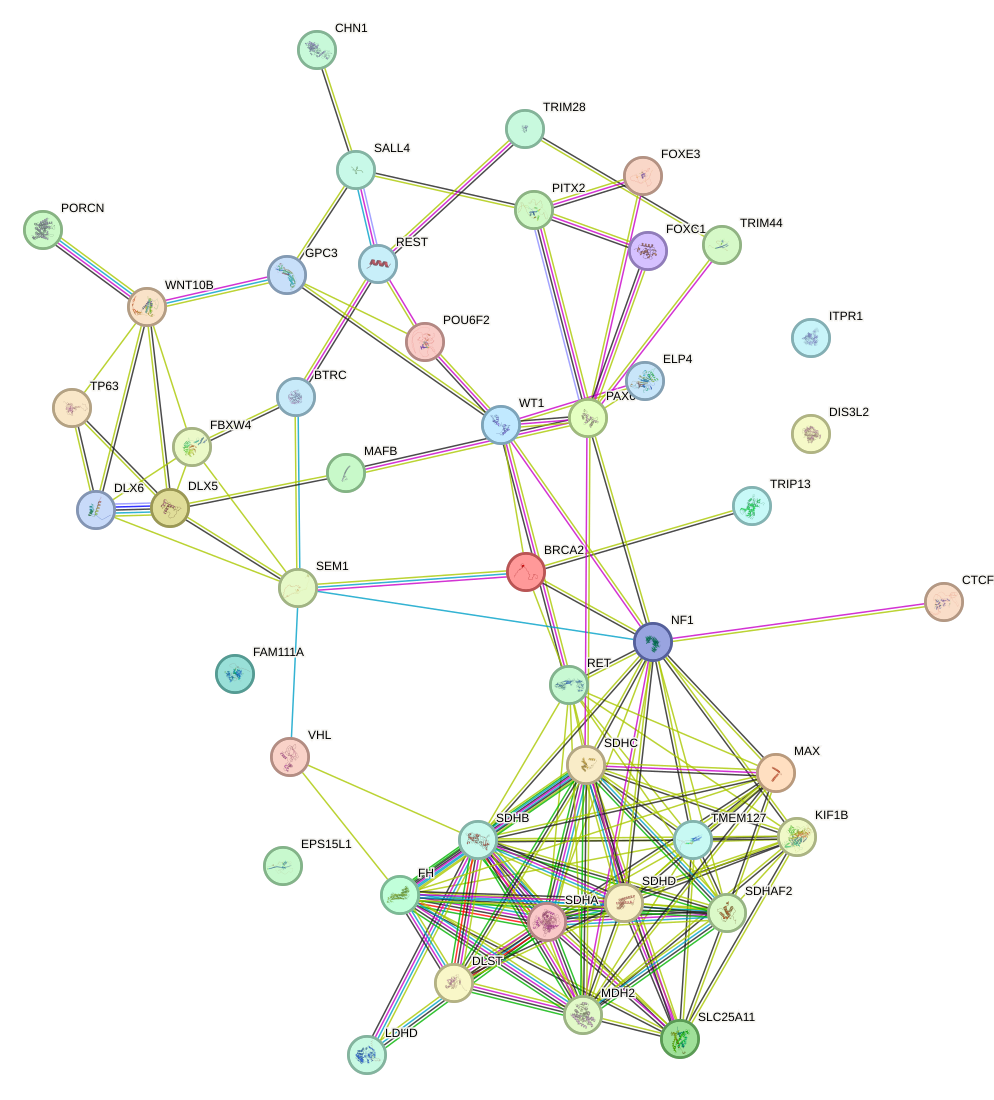
\includegraphics[width=1\textwidth]{figures/red_interaccion_aniridia.png} % Especifica la ruta y el tamaño
	\caption{Red de interacción con los genes asociados al fenotipo HP:0000526} % Agrega una leyenda si deseas
	\label{fig:mi-imagen} % Etiqueta para referenciar la imagen en el texto
\end{figure}

\subsection{Propagación de la red}

A partir de los genes semilla WNT10B, WT1, SEM1, PAX6, y NF1, se generó una red de interacciones proteína-proteína (PPI) utilizando datos de STRINGdb. Se estableció un umbral de puntaje de interacción de 700 para incluir únicamente conexiones de alta confianza. La red inicial centrada en los genes semilla fue posteriormente expandida mediante el algoritmo DIAMOnD, incluyendo 200 nodos adicionales que se encuentran altamente conectados con los genes semilla y entre sí.

La red generada señala importantes interacciones entre los genes semilla y otros desconocidos (como la relación WNT10B - TGFB2), lo cual permite continuar el estudio hacia el objetivo del artículo.


\subsection{Clustering}

\begin{figure}[!h] % [h] indica que queremos la imagen aquí, en la posición actual
	\centering
	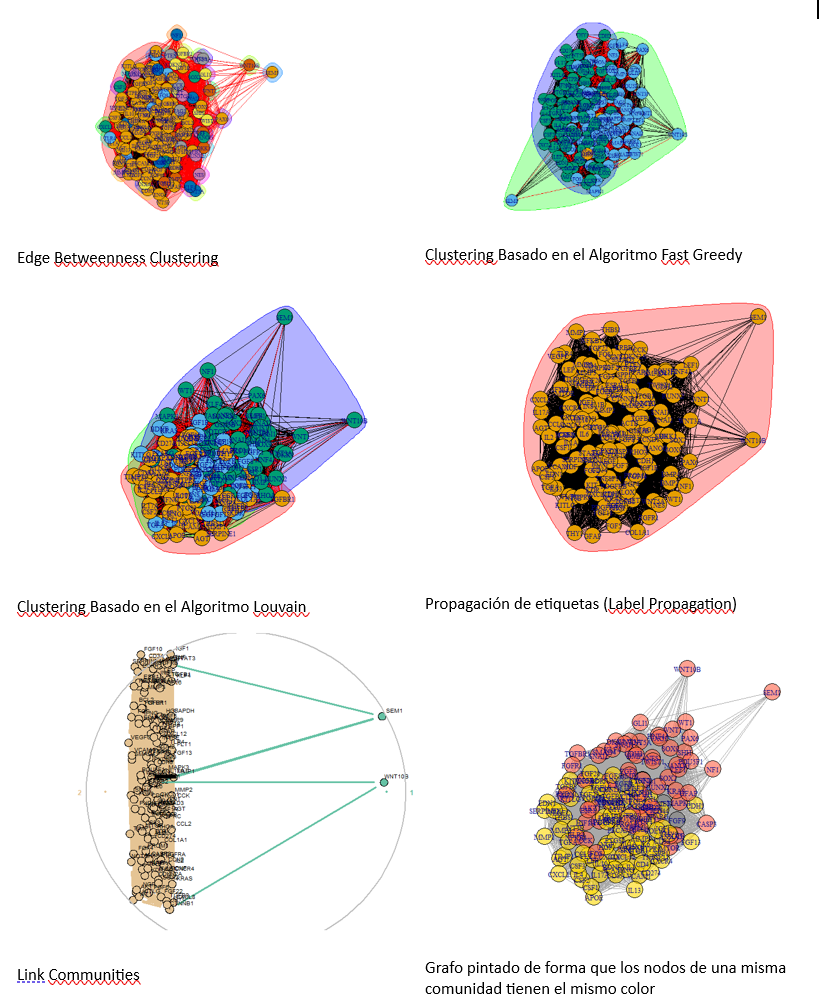
\includegraphics[width=1\textwidth]{figures/toda_figuras_clustering.png}
	\caption{Figuras obtenidas al aplicar clustering con distintos métodos}
	\label{clustering}
\end{figure}

Para esto usaremos la figura \ref{clustering}. Principalmente el estudio de los resultados se centrará en los genes semilla (WNT10B, WT1, SEM1, PAX6, NF1). En común, se puede observar que SEM1 aparece en varisa posiciones destacadas en los grafos; WT1 y PAX6 están en regiones densas (centrales) de las comunidades, lo que infica que tienen muchas conexiones internas; y NF1 se sitúa en los bordes de las comunidades, por lo que podría actuar como puente entre diferentes comunidades; y WNT10B también es central en algunas comunidades.


\subsection{Enriquecimiento y combinación de fenotipos}

Al realizar un análisis de enriquecimiento considerando la categoría “Process” generamos un archivo que nos permite comprender en qué procesos biológicos clave están involucrados los genes del cluster seleccionado. Esto ayuda a identificar rutas metabólicas, mecanismos celulares y funciones moleculares que pueden estar asociados con el fenotipo de interés.

Por otra parte, realizar el enriquecimiento funcional considerando categoría “HPO” es crucial para identificar cómo los genes analizados están asociados con características fenotípicas específicas, especialmente aquellas relacionadas con enfermedades humanas. 
Por último, combinar los fenotipos resultantes del enriquecimiento y los asociados a las enfermedades asociadas a nuestro fenotipo permite confirmar si los términos fenotípicos enriquecidos en los clusters tienen una relación directa con las enfermedades previamente identificadas. Si hay coincidencias, esto valida que los genes analizados están realmente relacionados con el fenotipo de interés.

Además, el establecer identificaciones entre las relaciones genotipo-fenotipo ayuda a establecer conexiones concretas entre los genes y las manifestaciones clínicas observadas en pacientes. Esto es especialmente útil para comprender cómo los genes influyen en el desarrollo de ciertas enfermedades o características clínicas.

Finalmente, podemos ver que 284 fenotipos de los 668 obtenidos tras el enriquecimiento están relacionados con enfermedades relacionadas con nuestro fenotipo a estudiar. Este resultado sugiere que el análisis de enriquecimiento funcional está capturando información biológica y clínica relevante. La conexión entre los fenotipos obtenidos y las enfermedades relacionadas con la aniridia valida que los genes analizados están efectivamente implicados en procesos relacionados con el fenotipo de interés. Este hallazgo podría abrir la puerta a la identificación de procesos centrales o vías moleculares críticas en estas enfermedades.
Por otra parte,  los fenotipos compartidos pueden ayudar a priorizar genes o grupos de genes específicos para estudios adicionales. Estos genes podrían ser considerados como potenciales biomarcadores o dianas terapéuticas para tratar tanto la aniridia como las enfermedades relacionadas.
Los fenotipos no relacionados también son interesantes, ya que podrían reflejar aspectos únicos del fenotipo de interés o nuevas áreas de estudio.





